\documentclass{article}

% The official NeurIPS 2026 style file was not available from the NeurIPS
% style-file URLs checked on 2026-07-04. This draft uses the official
% NeurIPS 2023 style as a temporary formatting placeholder; replace it with
% the 2026 style before a workshop submission if the 2026 file is released.
\usepackage[preprint]{neurips_2023}

\usepackage{booktabs}
\usepackage{graphicx}
\usepackage{hyperref}
\usepackage{microtype}
\usepackage{url}

\title{When Speculative Decoding Helps and Hurts: A Seed-Repeated GH200 Study of Qwen and Llama Model Pairs}

\author{%
  Taehoon Kang \\
  Independent Researcher \\
  \texttt{https://github.com/thkang091/DraftVerifyBench}
}

\begin{document}

\maketitle

\begin{abstract}
Speculative decoding is a well-established approach for accelerating transformer inference, but its latency benefit is conditional on the draft model, verifier model, workload, draft length, and serving backend.
This paper reports a reproducible empirical characterization of that conditionality on two draft--verifier pairs, Qwen2.5-0.5B-Instruct$\rightarrow$Qwen2.5-7B-Instruct and Llama-3.2-1B$\rightarrow$Llama-3.1-8B, measured on a single NVIDIA GH200 480GB system.
Across two seeds, five prompt classes, three temperatures, and four draft lengths, Qwen was consistently slower under the custom speculative decoder (mean $0.5936\times$, median $0.5826\times$), while Llama had positive mean speedup but negative median speedup (mean $1.0667\times$, median $0.8689\times$), with rare large wins reaching $12.8418\times$.
We validate a simple seed-held-out routing gate using only model family and oracle-labeled prompt type.
For Llama, the router improves expected speedup over an always-$k=4$ policy ($1.2294\times$ vs. $1.2068\times$) and reduces total slowdown rate (37.22\% vs. 45.00\%), while still losing on 53.17\% of the individual rows where it chooses speculation.
The contribution is not a new speculative decoding algorithm or a novel claim that performance is conditional; rather, it is a transparent, seed-repeated, cross-framework-checked measurement artifact and a small deployability test for a routing gate.
\end{abstract}

\section{Introduction}

Speculative decoding accelerates large language model inference by asking a smaller draft model to propose tokens and a larger verifier model to validate them.
Prior work has shown that this can reduce the number of expensive verifier forward passes while preserving the target distribution under the appropriate acceptance rule \cite{leviathan2022speculative,chen2023speculative}.
It is also well understood that the optimization is conditional: the draft model can be too slow, the verifier may not accept enough proposals, and backend overheads can erase theoretical wins.

This paper therefore does not claim to discover that speculative decoding is workload- or model-pair-dependent.
Instead, it asks a narrower systems question: on two concrete open model pairs and a fixed GPU platform, when does speculative decoding help, when does it fail, and can a simple held-out-seed router make a positive expected-value decision from pre-generation features?
The study uses DraftVerifyBench, a benchmark that records per-row latency, acceptance, verifier-call reduction, draft overhead, and hardware metadata.

The main findings are:
(1) Qwen2.5-0.5B-Instruct$\rightarrow$Qwen2.5-7B-Instruct was stably slower across both seeds and all aggregate prompt categories.
(2) Llama-3.2-1B$\rightarrow$Llama-3.1-8B exhibited a mean-vs.-median gap: large structured-workload wins lifted the mean above one, but the median speculative row remained slower than baseline.
(3) Draft length mattered: for Llama, $k=4$ and $k=8$ crossed median break-even, while $k=1$ and $k=2$ did not.
(4) A seed-held-out regime router improved expected value over always speculating at $k=4$, but it should be described as a risk-shaping gate, not as a classifier that avoids all losing cases.

\section{Related Work}

Speculative decoding was formalized for transformer inference by Leviathan, Kalman, and Matias \cite{leviathan2022speculative}, and speculative sampling for large language model decoding was developed by Chen et al. \cite{chen2023speculative}.
These works establish the core draft-and-verify mechanism and the distribution-preserving acceptance logic.
The present study uses a greedy custom decoder for characterization and explicitly does not claim exact stochastic speculative sampling.

Several later systems and algorithms extend the speculative decoding family.
SpecInfer explores tree-structured speculative inference and verification for serving \cite{miao2023specinfer}.
Staged speculative decoding studies multi-stage inference acceleration \cite{spector2023staged}.
Medusa attaches multiple decoding heads to accelerate generation without an external draft model \cite{cai2024medusa}, while EAGLE argues that feature uncertainty must be reconsidered in speculative sampling \cite{li2024eagle}.
PagedAttention and vLLM address memory management and high-throughput serving for LLM inference \cite{kwon2023pagedattention}; we include a small vLLM comparison to avoid evaluating only against the local decoder.

\section{Method}

\paragraph{Hardware and software.}
The GH200 experiments were run on a single NVIDIA GH200 480GB system with CUDA 13.0, NVIDIA driver 580.105.08, PyTorch 2.12.1+cu130, Transformers 5.12.1, and Python 3.12.3 on Linux-6.8.0-1046-nvidia-64k-aarch64.
All headline rows were run in bfloat16 with batch size 1 and CUDA timing synchronization.

\paragraph{Model pairs.}
We evaluate Qwen/Qwen2.5-0.5B-Instruct as draft for Qwen/Qwen2.5-7B-Instruct, and meta-llama/Llama-3.2-1B as draft for meta-llama/Llama-3.1-8B.
The committed metadata records approximately 0.494B and 7.616B parameters for the Qwen pair, and 1.236B and 8.030B parameters for the Llama pair.

\paragraph{Prompt taxonomy and grid.}
The full-static grid uses 15 prompts across five oracle-labeled prompt classes: code completion, structured JSON, factual QA, summarization, and open-ended generation.
Each model pair is evaluated for seeds 42 and 43, temperatures 0.0, 0.3, and 0.7, draft lengths $k \in \{1,2,4,8\}$, two repetitions, max-new-tokens 128, and one warmup prompt.
This yields 450 rows per model-pair seed run, or 1,800 total rows across both pairs and both seeds; 1,440 of those are speculative rows.

\paragraph{Decoder and metrics.}
The custom decoder implements greedy speculative decoding and records baseline latency, speculative latency, speedup versus baseline, acceptance rate, draft overhead, and verifier calls per output token.
Speedup is defined as baseline latency divided by speculative latency for the same prompt, temperature, repetition, and model pair.
Rows with nonzero temperature are timing diagnostics for the implementation; because exact stochastic speculative sampling with probability correction is not implemented, these rows should not be interpreted as distribution-preserving sampling claims.

\paragraph{Router validation.}
The router experiment converts each held-out seed into 90 validation cases per model family.
Each case has one baseline outcome and four candidate speculative outcomes ($k=1,2,4,8$).
For each held-out seed, the trained regime router selects an action using the opposite seed only and features available before generation: model family and oracle-labeled prompt type.
It does not use realized acceptance rate, realized speedup, latency, output text, or verifier-call counts for held-out decisions.
We compare the router against never speculate, always speculate at $k=4$, and a hindsight oracle that chooses the best per-row action after seeing outcomes.
The oracle is a ceiling, not a deployable policy.

\section{Results}

\subsection{Aggregate model-pair behavior}

Table~\ref{tab:model_pair} summarizes the two-seed speculative rows by model family.
The central result is not a single average speedup.
Qwen is a consistent loss, while Llama has a positive mean but negative median, indicating that large wins are concentrated in a minority of rows.

\begin{table}[t]
  \centering
  \caption{Two-seed GH200 full-static speculative results generated from committed per-row CSVs.}
  \label{tab:model_pair}
  \resizebox{\textwidth}{!}{\begin{tabular}{lllllll}
\toprule
Pair & Spec rows & Mean & Median & Best & Slowdown & Acceptance \\
\midrule
Llama 1B$\rightarrow$8B & 720 & 1.0667$\times$ & 0.8689$\times$ & 12.8418$\times$ & 67.36\% & 0.727 \\
Qwen 0.5B$\rightarrow$7B & 720 & 0.5936$\times$ & 0.5826$\times$ & 1.5739$\times$ & 99.17\% & 0.597 \\
\bottomrule
\end{tabular}
}
\end{table}

Figure~\ref{fig:draft} shows that the Llama mean-vs.-median story depends strongly on draft length.
For Llama, $k=4$ and $k=8$ cross median break-even, while $k=1$ and $k=2$ remain below median break-even.
Qwen remains below break-even for all draft lengths.

\begin{figure}[t]
  \centering
  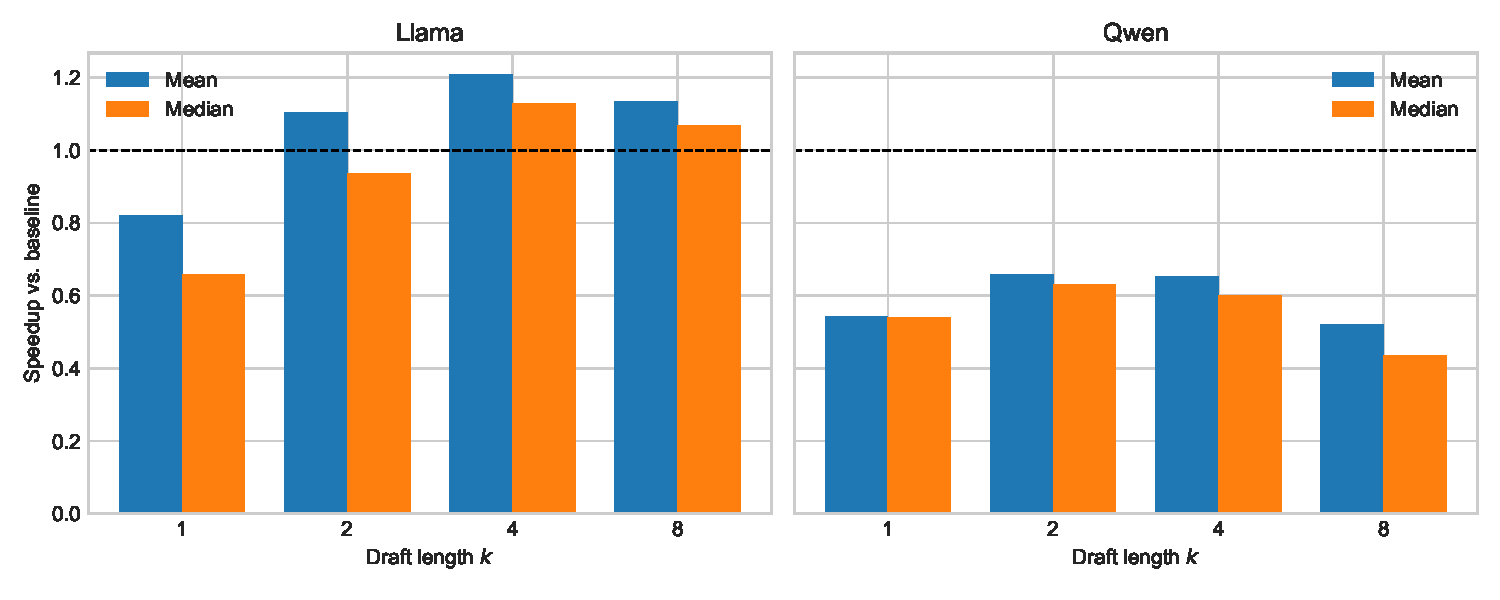
\includegraphics[width=0.95\textwidth]{figures/mean_median_by_draft_k.pdf}
  \caption{Mean and median speedup by draft length. Llama benefits concentrate at larger draft lengths; Qwen remains below break-even.}
  \label{fig:draft}
\end{figure}

\begin{table}[t]
  \centering
  \caption{Draft-length breakdown. Each row aggregates both seeds for one model family and draft length.}
  \label{tab:draft}
  \resizebox{\textwidth}{!}{\begin{tabular}{llllll}
\toprule
Pair & $k$ & Rows & Mean & Median & Slowdown \\
\midrule
Llama & 1 & 180 & 0.8210$\times$ & 0.6593$\times$ & 90.00\% \\
Llama & 2 & 180 & 1.1047$\times$ & 0.9360$\times$ & 88.33\% \\
Llama & 4 & 180 & 1.2068$\times$ & 1.1270$\times$ & 45.00\% \\
Llama & 8 & 180 & 1.1342$\times$ & 1.0675$\times$ & 46.11\% \\
Qwen & 1 & 180 & 0.5422$\times$ & 0.5401$\times$ & 100.00\% \\
Qwen & 2 & 180 & 0.6590$\times$ & 0.6315$\times$ & 98.89\% \\
Qwen & 4 & 180 & 0.6520$\times$ & 0.5994$\times$ & 98.89\% \\
Qwen & 8 & 180 & 0.5213$\times$ & 0.4345$\times$ & 98.89\% \\
\bottomrule
\end{tabular}
}
\end{table}

\subsection{Workload regimes}

Figure~\ref{fig:prompt} and Table~\ref{tab:prompt} show the workload-level regime structure.
For Llama, structured JSON has the largest mean speedup ($1.5408\times$), while summarization and code completion are near break-even on average and factual QA/open-ended are slower.
However, the structured JSON median is still below one ($0.8349\times$), so this category contains high-variance wins rather than uniformly fast rows.
For Qwen, every prompt class is slower on average and by median.

\begin{figure}[t]
  \centering
  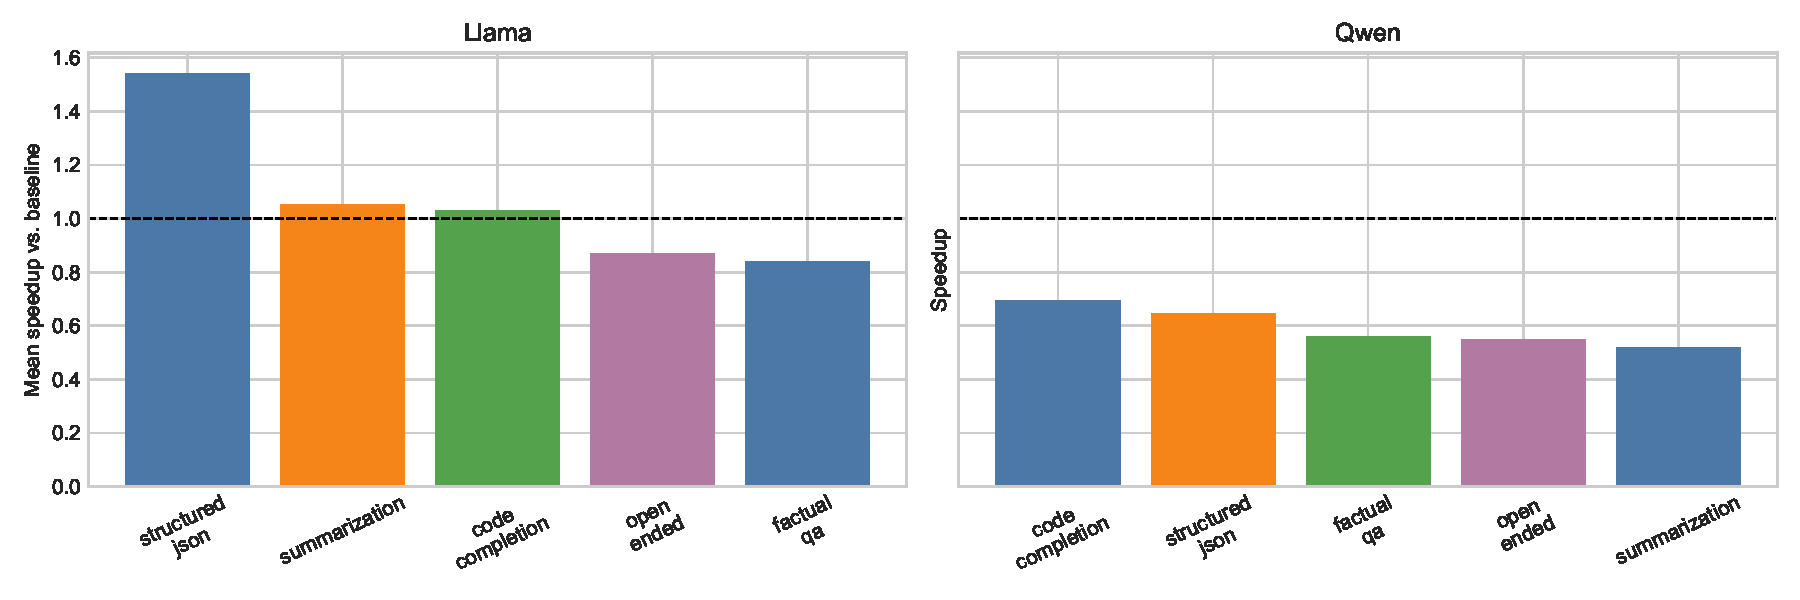
\includegraphics[width=0.95\textwidth]{figures/speedup_by_prompt_type.pdf}
  \caption{Mean speedup by oracle-labeled prompt type. The Llama result is a regime story; the Qwen result is broadly slower.}
  \label{fig:prompt}
\end{figure}

\begin{table}[t]
  \centering
  \caption{Prompt-type breakdown across both seeds.}
  \label{tab:prompt}
  \resizebox{\textwidth}{!}{\begin{tabular}{llllll}
\toprule
Pair & Prompt type & Rows & Mean & Median & Slowdown \\
\midrule
Llama & structured\_json & 144 & 1.5408$\times$ & 0.8349$\times$ & 63.19\% \\
Llama & summarization & 144 & 1.0520$\times$ & 0.9570$\times$ & 59.03\% \\
Llama & code\_completion & 144 & 1.0295$\times$ & 0.8776$\times$ & 64.58\% \\
Llama & open\_ended & 144 & 0.8702$\times$ & 0.9302$\times$ & 66.67\% \\
Llama & factual\_qa & 144 & 0.8411$\times$ & 0.7622$\times$ & 83.33\% \\
Qwen & code\_completion & 144 & 0.6930$\times$ & 0.6867$\times$ & 95.83\% \\
Qwen & structured\_json & 144 & 0.6467$\times$ & 0.6642$\times$ & 100.00\% \\
Qwen & factual\_qa & 144 & 0.5618$\times$ & 0.5542$\times$ & 100.00\% \\
Qwen & open\_ended & 144 & 0.5488$\times$ & 0.5561$\times$ & 100.00\% \\
Qwen & summarization & 144 & 0.5179$\times$ & 0.5380$\times$ & 100.00\% \\
\bottomrule
\end{tabular}
}
\end{table}

\subsection{Seed stability}

Table~\ref{tab:seed} and Figure~\ref{fig:seed} report seed-level aggregate stability.
Qwen is highly stable across seeds (mean $0.5938\times$ and $0.5935\times$).
Llama is less stable in the mean (seed 42 mean $1.1264\times$, seed 43 mean $1.0070\times$) but both seeds share the same qualitative pattern: median below one and rare large wins.
Two seeds are enough to catch an obvious one-run fluke; they are not enough for strong confidence intervals.

\begin{table}[t]
  \centering
  \caption{Seed-level speculative summaries.}
  \label{tab:seed}
  \resizebox{\textwidth}{!}{\begin{tabular}{lllllll}
\toprule
Pair & Seed & Rows & Mean & Median & Best & Slowdown \\
\midrule
Llama & 42 & 360 & 1.1264$\times$ & 0.8794$\times$ & 12.8418$\times$ & 66.11\% \\
Llama & 43 & 360 & 1.0070$\times$ & 0.8573$\times$ & 12.6823$\times$ & 68.61\% \\
Qwen & 42 & 360 & 0.5938$\times$ & 0.5818$\times$ & 1.5739$\times$ & 99.17\% \\
Qwen & 43 & 360 & 0.5935$\times$ & 0.5827$\times$ & 1.5378$\times$ & 99.17\% \\
\bottomrule
\end{tabular}
}
\end{table}

\begin{figure}[t]
  \centering
  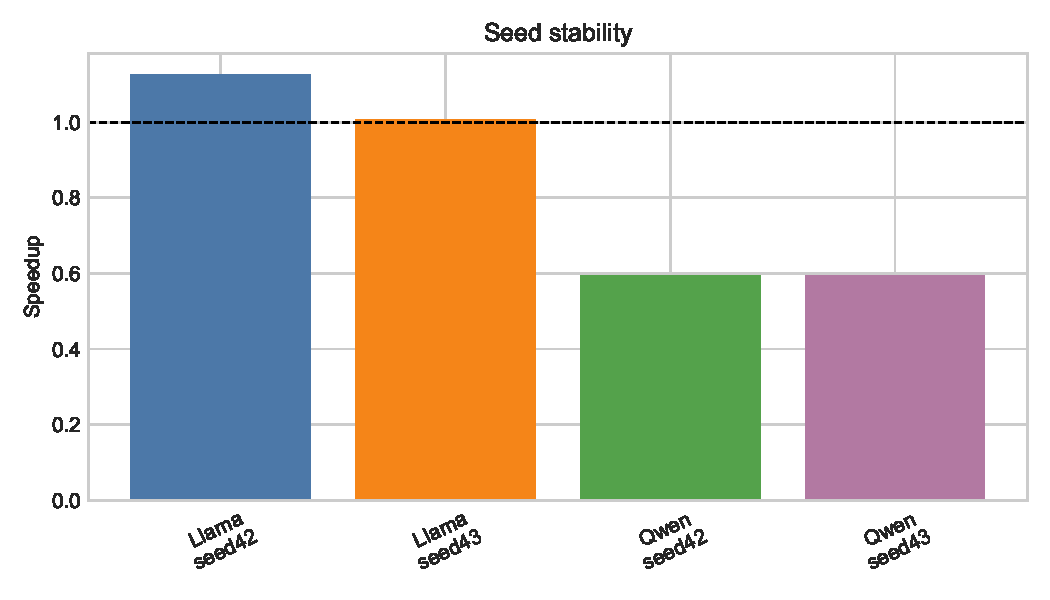
\includegraphics[width=0.75\textwidth]{figures/seed_stability.pdf}
  \caption{Mean speculative speedup by model family and seed.}
  \label{fig:seed}
\end{figure}

\subsection{Router validation}

Table~\ref{tab:router} and Figure~\ref{fig:router} compare routing policies on the held-out-seed cases.
For Llama, always speculating at $k=4$ achieves $1.2068\times$ mean speedup with a 45.00\% slowdown rate.
The trained regime router speculates on 70.00\% of validation cases, raises mean speedup to $1.2294\times$, and reduces total slowdown rate to 37.22\%.
Among only the rows where it chooses speculation, the conditional mean is $1.3277\times$.
At the same time, 53.17\% of those selected speculative rows still underperform baseline.
The correct interpretation is therefore expected-value-positive routing with large wins offsetting frequent small losses, not reliable avoidance of losing regimes.

The Llama oracle reaches $1.4363\times$ mean speedup.
The trained router captures 52.58\% of the available gain above never-speculate baseline:
\[
  \frac{1.2294 - 1.0000}{1.4363 - 1.0000} = 0.5258.
\]
For Qwen, the trained router selects baseline for every held-out validation case.
This is the correct expected-value decision for this grid, but it is not by itself evidence of a sophisticated within-family policy; the stronger router evidence is the Llama split.

\begin{table}[t]
  \centering
  \caption{Held-out-seed router validation. Rows are validation cases, not raw benchmark rows.}
  \label{tab:router}
  \resizebox{\textwidth}{!}{\begin{tabular}{llllllll}
\toprule
Pair & Policy & Rows & Mean & Slowdown & Spec share & Spec mean & Spec slowdown \\
\midrule
Llama & Never & 180 & 1.0000$\times$ & 0.00\% & 0.00\% & 1.0000$\times$ & 0.00\% \\
Llama & Always $k=4$ & 180 & 1.2068$\times$ & 45.00\% & 100.00\% & 1.2068$\times$ & 45.00\% \\
Llama & Trained router & 180 & 1.2294$\times$ & 37.22\% & 70.00\% & 1.3277$\times$ & 53.17\% \\
Llama & Oracle & 180 & 1.4363$\times$ & 0.00\% & 55.56\% & 1.7853$\times$ & 0.00\% \\
Qwen & Never & 180 & 1.0000$\times$ & 0.00\% & 0.00\% & 1.0000$\times$ & 0.00\% \\
Qwen & Always $k=4$ & 180 & 0.6520$\times$ & 98.89\% & 100.00\% & 0.6520$\times$ & 98.89\% \\
Qwen & Trained router & 180 & 1.0000$\times$ & 0.00\% & 0.00\% & 1.0000$\times$ & 0.00\% \\
Qwen & Oracle & 180 & 1.0062$\times$ & 0.00\% & 1.11\% & 1.5559$\times$ & 0.00\% \\
\bottomrule
\end{tabular}
}
\end{table}

\begin{figure}[t]
  \centering
  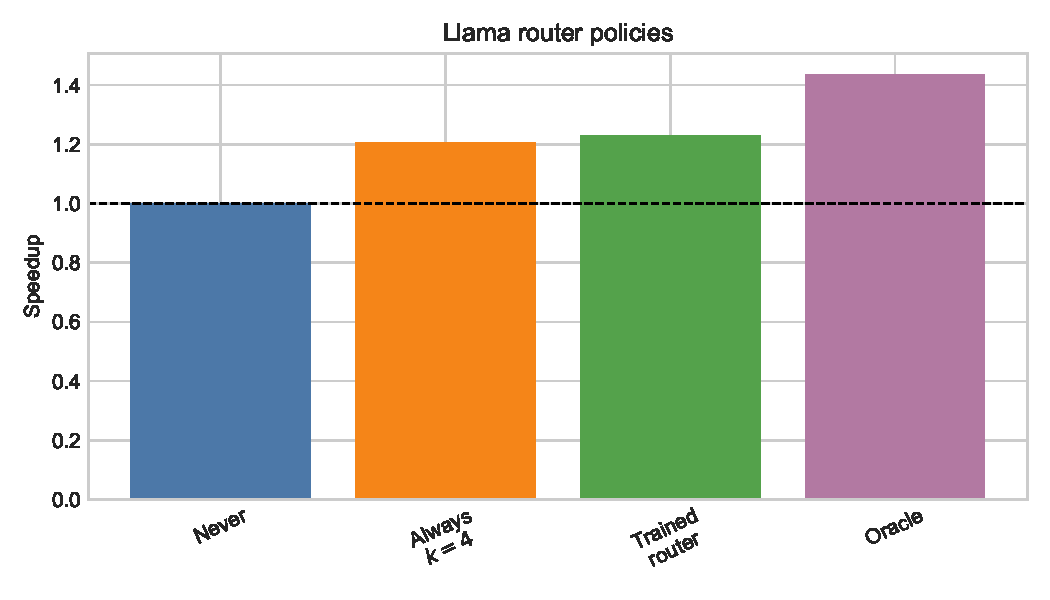
\includegraphics[width=0.75\textwidth]{figures/router_policy_comparison.pdf}
  \caption{Llama router policies. The trained router improves expected value over always-$k=4$ but remains below the hindsight oracle ceiling.}
  \label{fig:router}
\end{figure}

\subsection{Cross-framework checks}

Table~\ref{tab:framework} reports small cross-framework comparisons.
Hugging Face assisted generation was evaluated on nine assisted rows for each model pair.
It was slower on average for both pairs in this subset, with Llama mean speedup $0.8082\times$ and Qwen mean speedup $0.4735\times$ relative to Hugging Face generation.
The vLLM Llama speculative comparison over nine prompts was also slower in this configuration ($0.1247\times$), while the Qwen vLLM speculative run failed before generation because vLLM required the target and draft model vocabularies to match.
These comparisons are small and should be read as backend sanity checks, not as exhaustive serving benchmarks.

\begin{table}[t]
  \centering
  \caption{Small cross-framework comparisons generated from committed CSVs.}
  \label{tab:framework}
  \resizebox{\textwidth}{!}{\begin{tabular}{lllllll}
\toprule
Comparison & Rows/prompts & Mean speedup & Median & Best & Slowdown & Exact match / throughput \\
\midrule
Llama & 9 & 0.8082$\times$ & 0.7668$\times$ & 1.2423$\times$ & 77.78\% & 33.33\% \\
Qwen & 9 & 0.4735$\times$ & 0.4252$\times$ & 0.8707$\times$ & 100.00\% & 55.56\% \\
vLLM Llama & 9 & 0.1247$\times$ & -- & -- & 100.00\% & 164.2 tok/s vs. 1316.8 \\
\bottomrule
\end{tabular}
}
\end{table}

\section{Limitations}

Latency is hardware-dependent.
The headline Qwen/Llama timings were measured on one NVIDIA GH200 480GB instance; local GPT-2-family timing in the repository was measured separately on Apple MPS and is not used for the headline GH200 claims.
The prompt suite is intentionally small and synthetic, and the router uses oracle-labeled prompt types rather than a deployed prompt classifier.
Only two random seeds were run, which checks for obvious flukes but does not support strong confidence intervals.
The custom decoder implements and validates greedy speculative decoding only.
Exact stochastic speculative sampling with probability correction is not implemented, so nonzero-temperature speculative rows are diagnostic timing comparisons rather than exact distribution-preserving sampling results.
This is a local profiler and benchmark, not a production serving engine, and no GPU kernel-level optimization was implemented.
The Hugging Face assisted-generation and vLLM comparisons are small subsets and should not be generalized to all framework configurations.
The Qwen vLLM speculative comparison did not run because the target and draft vocabulary sizes differed.
Finally, these results should not be generalized beyond the specific model pairs, prompt suite, hardware, software versions, and decoder/backend configurations tested here.

\section{Code and Data Availability}

Code and committed result artifacts are available at \url{https://github.com/thkang091/DraftVerifyBench}.
The raw GH200 per-row CSVs used to regenerate every headline table in this paper are committed under \texttt{results/}.
The figures and tables in this draft are regenerated by \texttt{paper/generate\_assets.py}, which checks that required input CSVs are tracked by git.
The router table is regenerated directly from the raw full-static grids by \texttt{scripts/validate\_router\_from\_grid.py}.

\section{Conclusion}

On this GH200 study, speculative decoding is neither uniformly useful nor uniformly harmful.
Qwen2.5-0.5B$\rightarrow$7B was consistently slower, while Llama-3.2-1B$\rightarrow$Llama-3.1-8B produced rare large wins that lifted the mean above one despite a slower median row.
A simple held-out-seed router improved expected value and reduced total slowdown rate for Llama, but it still selected many losing speculative rows.
The practical takeaway is that speculative decoding should be profiled and gated by model pair and workload regime before deployment.

\bibliographystyle{plain}
\bibliography{references}

\end{document}
